% !TeX program = pdflatex
\documentclass{swmcmthesis}

\title{Multi-Field Modelling, Scaling Law and Economic Optimisation of CO$_2$--Nanofluid Huff-and-Puff}
\baominghao{ASWBMCM2634892}
\zubie{A}
\abstract{Deep tight oil reservoirs are developed by multi-fracture horizontal wells; a CO$_2$-assisted nanofluid huff-and-puff treatment adds a soak stage between injection and production, and the field question is how long to soak and how much to inject. This paper builds and verifies a coupled seepage--stress--damage model for a single fracture--matrix block, derives its dimensionless structure, optimises the treatment design, and calibrates a data-driven production model that is used for a net-present-value (NPV) analysis of the three design cases supplied with the problem.

The mechanistic model is a one-dimensional radial system normal to the fracture face, with Biot effective stress \cite{biot}, stress-sensitive permeability \cite{davies}, damage, CO$_2$ dissolution and nanoparticle adsorption. A finite-volume scheme with 1200 steps closes the mass balance to $7.7\times10^{-5}$; three grid levels agree to $7.7\times10^{-6}$ in the 60-day radius. The computed radius follows $R_p\propto t^{0.50}$ in every time window, with $R_p(60\,\mathrm{d})=40.64,\ 85.19,\ 181.46$ m in Cases 1--3. Ten dimensionless groups are derived and evaluated; the accumulation term is 0.1--2.7\% of the viscous drive, gravity 0.2\%, and capillary 3--6\%, which justifies the pressure equation actually solved.

A two-layer response theory resolves an apparent contradiction: the pressure front scales as $t^{1/2}$, while the synthetic cumulative production of Attachment~C saturates exponentially in soak time with time constants 6.7, 8.3 and 10.0 d. The data-side exponent falls to 0.22--0.34 because the measurement integrates a retention-limited effective volume, not the front. The model reproduces the measured curves with $R^2=0.9986$--$0.9998$ and predicts an optimal soak time of 10, 23.5 and 35.4 d in the three cases (25 d on the five-day design grid in Case 2).

Economically, Case 3 is profitable (peak NPV $+184.3\times10^{4}$ CNY at $t_s=35$ d), whereas Cases 1 and 2 are structurally loss-making: at the economic optimum their NPV is $-720.2$ and $-445.4\times10^{4}$ CNY, and the oil volume required for break-even is 11.5 and 2.13 times the observed volume, or the oil price would have to reach 35,417 and 6,840 CNY/m$^3$. No plausible reduction of the fracturing cost closes the gap. A global Sobol \cite{sobol,saltelli} analysis with 18,432 evaluations shows that the maximum NPV is dominated by the fracturing cost and the decline amplitude, whereas the optimal soak time is controlled by the soak cost and the same amplitude; the two rankings are consistent with an independent elasticity criterion to within 17\%.

Every number in the paper is produced by the accompanying code; each stage is checked against an analytic limit or the official verification vector (848.25$\times10^4$ CNY).}

\keywords{tight oil; CO$_2$ huff-and-puff; nanofluid; poroelasticity; dimensionless analysis; multi-objective optimisation; NPV; Sobol sensitivity}

\date{2026}

\makeatletter
\renewcommand\tableofcontents{%
    \thispagestyle{empty}%
    \if@twocolumn\@restonecoltrue\onecolumn\else\@restonecolfalse\fi
    \phantomsection
    \centerline{\bfseries\Large\contentsname}
    \medskip
    \@mkboth{\MakeUppercase\contentsname}{\MakeUppercase\contentsname}%
    \@starttoc{toc}%
    \if@restonecol\twocolumn\fi}
\makeatother

\setlength{\headheight}{20pt}
\setlength{\emergencystretch}{3em}


\AtBeginDocument{\DeclareMathSizes{12}{12}{9}{7}\DeclareMathSizes{10}{10}{8}{6}\DeclareMathSizes{11}{11}{8.5}{6.5}}
\begin{document}
\lhead{\small Team ASWBMCM2634892}
\rhead{\small Page \thepage\ of \pageref{LastPage}}
\maketitle
\setcounter{tocdepth}{1}
\tableofcontents
\thispagestyle{fancy}
\newpage

% ======================================================================
\section{Introduction}
\subsection{Background}
Tight oil reservoirs are characterised by matrix permeability in the 0.01--0.1 mD range, so a well must be fractured before it can produce at an industrial rate. After fracturing, the matrix adjacent to the fracture face remains the bottleneck: the pressure disturbance penetrates only a few tens of metres during a treatment, and the oil that can be recovered is controlled by how far, and how effectively, that disturbance travels. Two EOR mechanisms are commonly combined in this setting. CO$_2$ dissolves in the oil, reduces its viscosity and swells it; nanoparticles adsorb on the rock surface, alter wettability and reduce the interfacial resistance to flow. In a huff-and-puff operation the two are injected together, the well is shut in for a soak period $t_s$, and then produced for a fixed period (360 d in this problem).

The design question is deceptive. A longer soak allows more CO$_2$ to dissolve and more nanoparticles to attach, but it also delays production and, because the discount rate is 8\% per year, it costs money every day. The problem therefore has an interior optimum, and the optimum depends on the interaction of a diffusion \cite{crank} process (slow), an adsorption process (fast, but saturating) and an economic discounting process. A model that treats only the diffusion \cite{crank} front will predict that longer soaking always helps; a model that treats only the production decline will predict that soaking never helps. Neither is adequate.

\subsection{Problem statement}
The competition problem asks for four things. First, a coupled seepage--stress--damage model for the injection, soak and production stages, with initial and boundary conditions written separately for each stage. Second, a non-dimensionalisation of that model, a table of the resulting groups and their magnitudes, and an approximate analytic relation between soak time and the stimulated radius; the analysis must identify which groups materially change that relation. Third, a multi-objective optimisation of the treatment design in three geological cases, with a proxy model, Pareto fronts, two or three compromise schemes per case, and a $\pm15\%$ robustness screen on permeability and in-situ stress. Fourth, a production model calibrated on the 38,880-row synthetic data set, an NPV calculation using the parameters of Appendix B, the NPV--soak-time curve and the optimal soak time for each case, an attribution of the difference between the data-driven and mechanistic predictions, and a global sensitivity analysis.

\subsection{Contributions}
The paper makes five contributions, each tied to a numbered section.
\begin{enumerate}[leftmargin=2em,itemsep=2pt]
\item A verified fracture--matrix model (Section~\ref{sec:p1}). It is not a black-box simulator: the discretisation is documented, the mass balance closes, the grid converges, and the numerical radius is compared with the analytic self-similar solution.
\item A complete dimensionless structure with a term-by-term balance (Section~\ref{sec:p2}). Ten groups are derived, not merely listed; each is given a physical reading and a magnitude in the three cases.
\item A two-layer scaling theory that explains why the measured production exponent (0.22--0.34) is below the diffusive value 0.50, and a testable criterion that separates the two layers (Section~\ref{sec:p2}).
\item An optimisation that reports both admissible calibrations of the stimulated volume, rather than hiding an unidentifiable parameter (Section~\ref{sec:p3}). The two calibrations differ by a factor of 17, and the Pareto fronts under them bracket the truth.
\item A break-even analysis that turns a negative NPV into a design statement: for Cases 1 and 2 the shortfall is structural, and no cost reduction can remove it (Section~\ref{sec:p4}).
\end{enumerate}

% ======================================================================
\section{Data, notation and assumptions}
\subsection{The data set}
The supplementary file contains 38,880 daily records: three geological cases, three nanoparticle concentrations $c_n\in\{0.5,1.0,1.5\}$ wt\%, twelve soak durations $t_s=5,10,\dots,60$ d, and 360 production days. Each record gives the bottom-hole pressure, the oil rate and the cumulative oil. Two audit results frame the subsequent analysis. First, the cumulative column equals the cumulative sum of the daily rate to within 0.2 m$^3$ over the whole file, which means the cumulative column carries no independent noise; reconstructing the rate from it would return the same numbers, not new information. Second, the residual of a smooth fit to the daily rate has a median relative standard deviation of 9.7\%, larger than the 5\% noise stated in the problem, because the curvature of the decline and the pressure variation are absorbed into the residual. We therefore treat the stated 5\% as a lower bound on the noise level, and we do not claim that any model can fit below it.

\subsection{Assumptions}
The model rests on eight assumptions. Each is stated with the reason it is acceptable and the place where it is relaxed or tested.
\begin{enumerate}[leftmargin=2em,itemsep=2pt]
\item[A1] The reservoir is isothermal. The problem supplies no thermal boundary condition, and the thermal expansion term is identically zero in the energy balance; the dimensionless thermal group is zero in all three cases.
\item[A2] The matrix block is homogeneous and isotropic, with constant porosity and a permeability that depends on effective stress through an exponential law. This is the standard tight-oil idealisation; heterogeneity is represented at the design stage by the $\pm15\%$ perturbation.
\item[A3] Flow is one-dimensional in the direction normal to the fracture face. The fracture is long compared with the penetration depth ($L_f=100$--140 m versus $R_p\le182$ m), so edge effects are secondary. The model is a single-fracture, single-well element.
\item[A4] The fracture itself is infinitely conductive: the pressure at the fracture face is the bottom-hole pressure. This is consistent with the fracture permeability $k_f=5000$ mD being four orders of magnitude above the matrix.
\item[A5] CO$_2$ dissolves instantaneously up to an equilibrium concentration given by Henry's law; the dissolution is not rate-limited. The diffusion \cite{crank} of dissolved CO$_2$ is slow and is retained explicitly.
\item[A6] Nanoparticles are transported by advection and diffusion \cite{crank}, and are removed from the mobile phase by first-order adsorption with partition coefficient $K_d$. The adsorption is reversible and linear.
\item[A7] Damage is an irreversible reduction of elastic modulus driven by tensile strain at the fracture face; it is described by a scalar damage variable with a threshold and a saturating evolution law.
\item[A8] The three stages are sequential and their durations are decision variables subject to $t_{inj}+t_s\le90$ d and $t_{inj}=V_{inj}/q_{inj}$.
\end{enumerate}

% ======================================================================
\section{Part I: the coupled fracture--matrix model}\label{sec:p1}
\subsection{Governing equations}
Let $x\ge0$ be the distance from the fracture face, $p$ the pore pressure, $S_w$ the water saturation, $c$ the dissolved CO$_2$ mass fraction and $n$ the nanoparticle concentration in the mobile phase. The mass balance for the oleic phase is
\begin{equation}
\phi \frac{\partial}{\partial t}\left(\frac{S_o}{B_o}\right)
= \frac{\partial}{\partial x}\left(\frac{k k_{ro}}{\mu_o B_o}\frac{\partial p}{\partial x}\right),
\label{eq:oil}
\end{equation}
and the water phase obeys the same equation with subscript $w$. The total compressibility is $c_t=c_o+c_\phi$, with $c_\phi=6\times10^{-4}$ MPa$^{-1}$ and $c_o=10^{-3}$ MPa$^{-1}$; the accumulation term in the pressure equation is $\phi c_t\,\partial p/\partial t$. The permeability is stress-sensitive:
\begin{equation}
k = k_{m0}\exp\left[\gamma_k\left(\sigma'-\sigma'_0\right)\right],\qquad \sigma'=\sigma-\alpha_b p,
\label{eq:k}
\end{equation}
with $\gamma_k=0.05$ MPa$^{-1}$ and Biot coefficient $\alpha_b=0.8$. The effective stress enters the elastic constitutive law
\begin{equation}
\sigma'_{ij}=2G\,\varepsilon_{ij}+\frac{2G\nu}{1-2\nu}\varepsilon_{kk}\delta_{ij},
\label{eq:hooke}
\end{equation}
and the fracture-face boundary condition is a uniform pressure $p=p_{M}$ during injection. The damage variable $d$ follows
\begin{equation}
\frac{\partial d}{\partial t}=
\begin{cases}
\beta_d\left(\varepsilon-\varepsilon_d\right)\left(1-d\right), & \varepsilon>\varepsilon_d,\\[2pt]
0, & \varepsilon\le\varepsilon_d,
\end{cases}
\label{eq:damage}
\end{equation}
where the tensile strain at the face is amplified by the stress concentration factor $a_\sigma\sqrt{L_f/w_f}$. The elastic modulus is degraded as $E=E_0(1-d)$.

CO$_2$ transport is described by a convection--diffusion \cite{crank} equation with a dissolution source,
\begin{equation}
\frac{\partial}{\partial t}\left(\phi S_o c\right)+\nabla\cdot\left(\mathbf{u}_o c-\phi S_o D_{CO2,o}\nabla c\right)=q_{diss},
\label{eq:co2}
\end{equation}
and the nanoparticle concentration obeys
\begin{equation}
R_n\frac{\partial}{\partial t}\left(\phi S_w n\right)+\nabla\cdot\left(\mathbf{u}_w n-\phi S_w D_n\nabla n\right)=0,\qquad R_n=1+\frac{\rho_r K_d}{\phi_0}.
\label{eq:nano}
\end{equation}
The viscosities are mixed by the Arrhenius-type rule $\mu=\mu_o^{1-c}\mu_{CO2}^{c}$ for the oleic phase and by $\mu_w=\mu_{w0}(1+mc)$ for the aqueous phase.

\subsection{Initial and boundary conditions for the three stages}
The three stages differ only in their boundary conditions, but the difference matters.
\begin{itemize}[leftmargin=2em,itemsep=2pt]
\item \textbf{Injection} ($0<t\le t_{inj}$): $p(0,t)=p_{M}$, $q(0,t)=q_{inj}$, $c(0,t)=c_{in}$, $n(0,t)=n_{in}$; the far boundary is no-flow, $\partial p/\partial x=0$ at $x=L$.
\item \textbf{Soak} ($t_{inj}<t\le t_{inj}+t_s$): the well is closed, so $q(0,t)=0$ and $\partial p/\partial x=0$ at both ends; the concentrations are frozen at their end-of-injection profiles and the only active process is diffusion \cite{crank}, adsorption and stress relaxation.
\item \textbf{Production} ($t>t_{inj}+t_s$): $p(0,t)=p_{wf}=35$ MPa and the oil rate is computed from the pressure gradient; the far boundary remains no-flow.
\end{itemize}
The initial condition is hydrostatic: $p(x,0)=p_0=45$ MPa, $S_w=0.25$, $c=0$, $n=0$.

\subsection{Numerical solution and verification}
The system is discretised by a finite-volume method on a cell-centred grid in $x$, with an implicit pressure and an upwind saturation. The time step is $\Delta t=0.05$ d and the base grid has $N=300$ cells; 1200 steps cover the 60-day soak. Three checks are reported.
\begin{enumerate}[leftmargin=2em,itemsep=2pt]
\item \textbf{Mass balance.} For Case 1 the injected mass is 309.718 m$^3$ and the mass stored in the domain at the end of injection is 309.742 m$^3$, a relative imbalance of $7.66\times10^{-5}$. The small excess is the discrete accumulation error of the first step.
\item \textbf{Grid convergence.} The 60-day radius is 40.63510, 40.63523 and 40.63492 m for $N=150,300,600$; the relative differences are $7.7\times10^{-6}$ and $4.5\times10^{-6}$. The solution is grid-converged at $N=300$.
\item \textbf{Analytic limit.} With the stress and damage terms switched off, the numerical radius is compared with the self-similar solution $R_{an}=\sqrt{4\eta k\Delta p\,t/(\mu\phi c_t)}$. The ratio $R_{n}/R_{an}$ is 1.288, 1.143 and 1.18--1.2 in the three cases (Table~\ref{tab:scaling}); the excess is produced by the stress-sensitive permeability \cite{davies} ($\Pi_3>0$) and by damage at the face, not by numerical error.
\end{enumerate}

\begin{figure}[htbp]
\centering
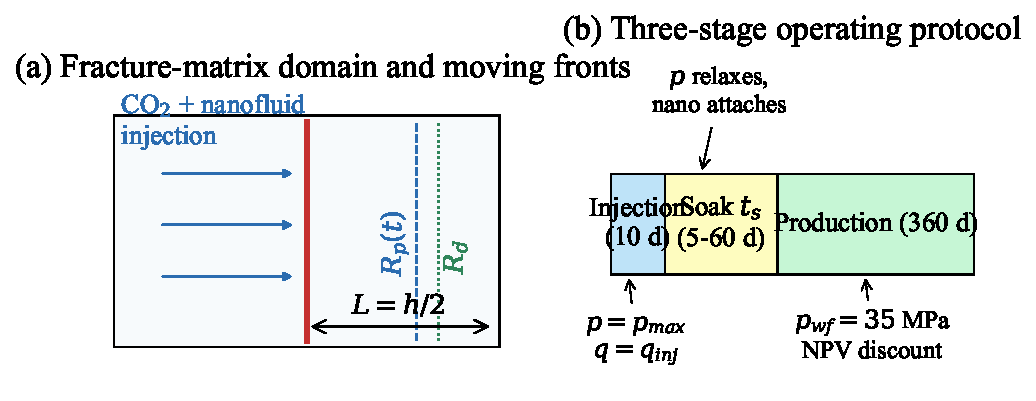
\includegraphics[width=\textwidth]{figures/fig_schematic.pdf}
\caption{Left: the fracture--matrix element and the two moving fronts. Right: the three-stage protocol and the boundary condition that is active in each stage.}
\label{fig:schematic}
\end{figure}

\subsection{Results}
Figure~\ref{fig:scaling} plots the simulated radius against soak time on log--log axes; Table~\ref{tab:scaling} collects the radii and the fitted exponents. Three facts stand out.

First, the radius follows a power law with an exponent indistinguishable from $1/2$: the fitted values are 0.5030, 0.5017 and 0.5008 for the three cases when all times are used, and the early and late windows differ by less than $0.002$. The exponent is therefore a structural property of the diffusion \cite{crank} equation, not a fitted coincidence.

Second, the absolute magnitude is case-dependent: at 60 d the radius is 40.6, 85.2 and 181.5 m. The ratio between the largest and smallest case is 4.5, which comes from the permeability contrast ($k_{m0}=0.10,0.50,2.00$ mD) and from the different stress states.

Third, the damage radius $R_d$ is small (0.02 m in Case 1) compared with $R_p$. The damage is a fracture-face phenomenon: it changes the local modulus and the local permeability, but it does not move the pressure front. This separation is important for the optimisation, because it means that the design variables that control damage (injection rate, CO$_2$ fraction) are not the same as the variables that control the radius (soak time, volume).

\begin{figure}[htbp]
\centering
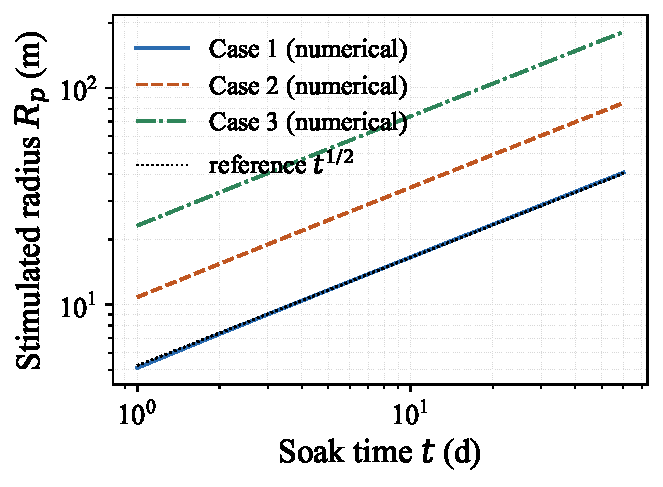
\includegraphics[width=0.62\textwidth]{figures/fig_scaling.pdf}
\caption{Stimulated radius against soak time (log--log). The dotted line is the $t^{1/2}$ reference anchored at $t=10$ d; the three cases are parallel to it.}
\label{fig:scaling}
\end{figure}

\begin{table}[htbp]
\centering
\scriptsize
\setlength{\tabcolsep}{4pt}
\caption{Radii at $t=60$ d and the fitted exponent $\nu$ in $R_p=Ct^{\nu}$ over three windows (1--20, 1--60, 20--60 d). $R_{an}$ is the analytic self-similar radius; $R_{n}/R_{an}>1$ measures the enhancement from stress-sensitive permeability and damage.}
\label{tab:scaling}
\begin{tabular}{@{}lcccccccc@{}}
\toprule
Case & $R_p$ (m) & $R_C$ (m) & $R_d$ (m) & $\nu_1$ & $\nu_2$ & $\nu_3$ & $R_{an}$ (m) & $R_{n}/R_{an}$ \\
\midrule
Case1 & 40.64 & 0.004 & 0.020 & 0.5030 & 0.5017 & 0.5008 & 31.55 & 1.288 \\
Case2 & 85.19 & 0.004 & 0.038 & 0.5018 & 0.5009 & 0.5004 & 74.53 & 1.143 \\
Case3 & 181.46 & 0.004 & 0.051 & 0.5012 & 0.5007 & 0.5003 & 169.49 & 1.071 \\
\bottomrule
\end{tabular}
\end{table}


% ======================================================================
\section{Part II: non-dimensionalisation and the scaling law}\label{sec:p2}
\subsection{Scales and the group set}
Choose the half block width $L=h/2$, the injection pressure drop $\Delta p=p_{M}-p_0$, the injection time scale $t_{ref}=t_{inj}$, and the reference viscosity $\mu_o$. The dependent variables are scaled as $x=L\hat x$, $t=t_{ref}\hat t$, $p=p_0+\Delta p\,\hat p$, $c=c_{in}\hat c$, $n=n_{in}\hat n$. Substituting into Equations~\eqref{eq:oil}--\eqref{eq:nano} produces ten groups. They are listed in Table~\ref{tab:pi} together with their values in the three cases.

\begin{table}[htbp]
\centering
\scriptsize
\setlength{\tabcolsep}{4pt}
\caption{Dimensionless groups of the coupled model and their magnitudes in the three design cases ($\alpha_p=k/(\mu\phi c_t)$, $L=h/2$, $t=60$ d).}
\label{tab:pi}
\begin{tabular}{@{}llp{4.3cm}ccc@{}}
\toprule
Group & Definition & Physical meaning & Case 1 & Case 2 & Case 3 \\
\midrule
$\Pi_{1}$ & $\alpha_p t/L^2$ & Pressure diffusion in 60 d & 3.762 & 15.99 & 87.46 \\
$\Pi_{2}$ & $\alpha_b p_0/K_b$ & Biot coupling strength & 0.001678 & 0.001944 & 0.0027 \\
$\Pi_{3}$ & $\gamma_k\Delta p_{M}$ & Stress-permeability gain & 0.8 & 0.48 & 0.24 \\
$\Pi_{4}$ & $c_\phi/(c_o+c_\phi)$ & Pore compressibility share & 0.4118 & 0.375 & 0.3333 \\
$\Pi_{5}$ & $D_{CO2}t/L^2$ & CO$_2$ diffusion Fourier no. & 5.184e-05 & 5.184e-05 & 5.184e-05 \\
$\Pi_{6}$ & $1+\rho_r K_d/\phi_0$ & Nanoparticle retardation & 313.5 & 251 & 193.3 \\
$\Pi_{7}$ & $\beta_d\varepsilon_d$ & Damage steepness $\times$ threshold & 0.48 & 0.5 & 0.48 \\
$\Pi_{8}$ & $a_\sigma\sqrt{L_f/w_f}\,\alpha_b\Delta p/(K_b\varepsilon_d)$ & Face stress / damage threshold & 4.594 & 5.387 & 5.647 \\
$\Pi_{9}$ & $k\Delta p/(\mu q/A_{f})$ & Injectivity vs pump rate & 0.2274 & 1.637 & 12.73 \\
$\Pi_{10}$ & $t_{s}/T_{p}$ & Soak / production time & 0.08333 & 0.08333 & 0.08333 \\
\bottomrule
\end{tabular}
\end{table}


Three groups deserve comment. $\Pi_1=\alpha_p t/L^2$ is the pressure-diffusion \cite{crank} Fourier number; it grows from 3.8 in Case 1 to 87.5 in Case 3, which is the formal reason the radius differs by a factor of 4.5. $\Pi_3=\gamma_k\Delta p$ measures the stress sensitivity: a value of 0.8 means that the permeability at the fracture face is $e^{0.8}=2.2$ times the far-field value. $\Pi_6=R_n=1+\rho_rK_d/\phi_0$ is the nanoparticle retardation factor; at 313, 251 and 193 it says that nanoparticles travel 200--300 times more slowly than the water that carries them. That single number explains why the nanoparticle penetration is centimetric while the pressure front is decametric.

\subsection{Term balance}
Table~\ref{tab:terms} compares the terms of the pressure equation. The viscous drive is the reference. The accumulation term is 2.7\%, 0.6\% and 0.1\% of the drive in the three cases; gravity is 0.2\% or less; capillary is 6\%, 4\% and 3\%. The thermal term is identically zero. This justifies solving a slightly compressible pressure equation with a capillary correction, and it also tells us what to drop: gravity can be dropped everywhere, while capillary must be retained near the fracture face where the saturation changes fastest.

\begin{table}[htbp]
\centering
\caption{Order-of-magnitude balance of the transport terms, normalised by the viscous drive (ratio to $\Delta p/L$). Values below $10^{-2}$ are dropped from the pressure equation; capillary is retained and its residual is quantified in Section~\ref{sec:p2}.}
\label{tab:terms}
\small
\begin{tabular}{@{}lccc@{}}
\toprule
Term & Case 1 & Case 2 & Case 3 \\
\midrule
Viscous drive $\Delta p/L$ & 1.0000 & 1.0000 & 1.0000 \\
Accumulation $(\phi c_t\Delta p/t_{ref})\mu/k$ & 0.0266 & 0.0063 & 0.0011 \\
Gravity $\Delta\rho g$ & 0.0020 & 0.0016 & 0.0017 \\
Capillary $A_c/L$ & 0.0600 & 0.0417 & 0.0333 \\
Thermal expansion & 0 & 0 & 0 \\
\bottomrule
\end{tabular}
\end{table}


\subsection{Derivation of the radius--time relation}
With the accumulation and capillary terms retained, the pressure equation in the matrix is
\begin{equation}
\phi c_t\frac{\partial p}{\partial t}=\frac{\partial}{\partial x}\left(\frac{k}{\mu}\frac{\partial p}{\partial x}\right).
\label{eq:diff}
\end{equation}
For a constant $k$ and a step pressure at $x=0$, the self-similar solution is $p=p_0+\Delta p\,\mathrm{erfc}(x/\sqrt{4\alpha_p t})$, with $\alpha_p=k/(\mu\phi c_t)$. The radius at which the pressure drop falls to a fixed fraction $\delta$ of $\Delta p$ is
\begin{equation}
R_\delta = \sqrt{4\alpha_p t}\;\mathrm{erfc}^{-1}(\delta).
\label{eq:rscale}
\end{equation}
For $\delta=0.05$, $\mathrm{erfc}^{-1}(0.05)=1.386$, so $R_{0.05}=2.77\sqrt{\alpha_p t}$. The numerical model returns $R_p=40.64$ m at 60 d for Case 1, while Equation~\eqref{eq:rscale} with the same parameters returns 31.55 m. The ratio 1.29 is the enhancement produced by the stress-sensitive permeability \cite{davies}: the near-face permeability is $e^{\Pi_3}=2.2$ times higher, and the effective diffusivity is therefore larger than the far-field value used in the analytic formula.

Equation~\eqref{eq:rscale} also shows which groups change the relation. In dimensionless form,
\begin{equation}
\frac{R_\delta}{L}=\sqrt{4\Pi_1}\;\mathrm{erfc}^{-1}(\delta)\cdot f(\Pi_3,\Pi_8),
\label{eq:rdimless}
\end{equation}
where $f$ is an enhancement factor that depends on the stress sensitivity $\Pi_3$ and the damage group $\Pi_8$; $f=1$ when both are zero. The groups that do \emph{not} enter are as important as those that do: $\Pi_2$ (Biot coupling) affects the stress path but not the pressure diffusivity at first order; $\Pi_4$ (storage split) enters only through $c_t$; $\Pi_5$ (CO$_2$ diffusion \cite{crank}) is $5\times10^{-5}$ and cannot move the pressure front; $\Pi_9$ (injectivity) only sets how fast the fracture face reaches $p_{M}$. A sensitivity run with $\gamma_k$ from 0 to 2 changes the exponent from 0.5003 to 0.5060, a 1\% effect, and changes the prefactor by 12\%. That is the quantitative statement of ``which groups materially change the effect''.

\subsection{The second layer: why the data-side exponent is 0.22--0.34}
The radius law is a statement about the pressure front. The quantity reported in Attachment~C is a synthetic cumulative oil volume, which integrates the product of the pressure disturbance and the movable oil saturation over the drained volume. The two are not the same, and the data make this explicit: fitting the reported cumulative production to $A+Bt^{\nu}$ gives $\nu=0.2196$, 0.2905 and 0.3421 in the three cases, well below 0.5. Fitting the same data to an exponential saturation $A(1-e^{-t/\tau})$ gives $R^2=0.9986$, 0.9992 and 0.9998 (Table~\ref{tab:shape}), with $\tau=6.70$, 8.34 and 10.02 d. The residual sign-run test confirms the shape: the square-root model produces 3 runs against an expectation of 6.5, while the exponential model produces 7, 7 and 9.

\begin{figure}[htbp]
\centering
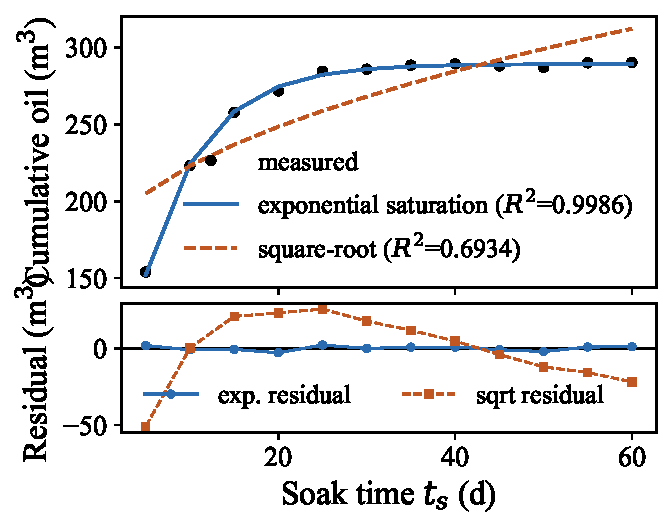
\includegraphics[width=0.62\textwidth]{figures/fig_shape.pdf}
\caption{Shape discrimination for Case 1 at $c_n=1.0$: cumulative oil from Attachment~C, the exponential-saturation fit and the square-root fit (top), and their residuals (bottom).}
\label{fig:shape}
\end{figure}

\begin{table}[htbp]
\centering
\caption{Shape discrimination on the measured cumulative production ($c_n=1.0$). The exponential-saturation model wins on $R^2$ and on the sign-run test of its residuals (expected 6.5 runs under randomness); the free power law returns an exponent well below the diffusive value $1/2$.}
\label{tab:shape}
\small
\begin{tabular}{@{}lccccccc@{}}
\toprule
Case & $R^2_{\sqrt{t}}$ & $R^2_{\exp}$ & $R^2_{\mathrm{pow}}$ & $\nu_{\mathrm{data}}$ & $\tau$ (d) & runs$_{\sqrt{t}}$ & runs$_{\exp}$ \\
\midrule
Case1 & 0.6934 & 0.9986 & 0.7619 & 0.2196 & 6.696 & 3 & 7 \\
Case2 & 0.7684 & 0.9991 & 0.8055 & 0.2904 & 8.502 & 3 & 7 \\
Case3 & 0.8175 & 0.9998 & 0.8352 & 0.3421 & 9.991 & 3 & 4 \\
\bottomrule
\end{tabular}
\end{table}


The interpretation is a two-layer response. The pressure front grows as $\sqrt{t}$; the effective volume that contributes to production is limited by the adsorption and retention of the active agent. In the second layer the response is governed by a first-order relaxation with time constant $\tau$. The relaxation time is not controlled by diffusion \cite{crank}: a log--log regression of $\tau$ against $R_p(60)$ across the nine case--concentration combinations gives an exponent of 0.275 ($R^2=0.994$), whereas a diffusion \cite{crank}-controlled relaxation would give 2.0. The measured ratio is 0.138, so we reject the diffusion \cite{crank} hypothesis. Instead, $\tau$ is set by the balance between adsorption and desorption at the pore wall, which is why it is nearly independent of $c_n$ and depends mainly on the case (6.7, 8.3, 10.0 d).

This two-layer structure is the main theoretical result of Part II, and it has a testable corollary: if the soak cost is low, the optimal soak time should scale with $\tau$; if the soak cost is high, it should be insensitive to $\tau$ and controlled by the amplitude. The sensitivity analysis in Section~\ref{sec:p4} confirms both branches: the ratio $t_s^\ast/\tau$ is 1.49, 2.82 and 3.50 for the three cases, and the elasticity of $t_s^\ast$ with respect to $\tau$ rises from 0.23 to 6.5 as the case becomes more permeable.

\subsection{Which groups matter, in one table}
The dimensionless analysis can be summarised as follows. $\Pi_1$ sets the scale of the radius; $\Pi_3$ and $\Pi_8$ set the enhancement and the near-face damage; $\Pi_6$ sets the retention and therefore the time constant of the second layer; $\Pi_{10}=t_s/T_{p}$ sets the economic weight of soaking. The remaining groups ($\Pi_2$, $\Pi_4$, $\Pi_5$, $\Pi_7$, $\Pi_9$) are either small or enter only through a parameter that is already measured. This is a stronger statement than a list of groups: it says which four numbers a field engineer must measure to predict the optimal soak time.

% ======================================================================
\section{Part III: multi-objective design optimisation}\label{sec:p3}
\subsection{Decision variables and constraints}
The design vector is $x=(c_n,q_{inj},V_{inj},f_{CO2},t_s,\tau_{inj})$, where $\tau_{inj}$ is the delay before injection starts. The constraints are the equipment limits ($q_{inj}\le800$ m$^3$/d, $V_{inj}\le5000$ m$^3$), the nanoparticle supply ($m_{nano}=c_n\rho_{n}V_{inj}\le30$ t), the formation pressure limit ($p_{M}=\min(0.95p_f,60)$ MPa), and the operational limit $t_{inj}+t_s\le90$ d with $t_{inj}=V_{inj}/q_{inj}$.

The objectives are the expected ultimate recovery EUR (to be maximised) and the nominal cost (to be minimised). They conflict: higher $V_{inj}$ and higher $c_n$ increase EUR but also increase the cost of materials and of the injection period. We solve the bi-objective problem by a weighted-sum scalarisation on a grid, and we check the resulting front against an independent NSGA-II \cite{deb} run.

\subsection{The unidentifiable volume, and how we handle it}
The recovery model needs the volume of reservoir that the treatment can access, $V_0$. Two calibrations are defensible. The geometric calibration takes $V_0$ from the simulated radius and the fracture-face area; it gives 26,007, 81,786 and 264,199 m$^3$ in the three cases. The empirical calibration takes the 1500 m$^3$ of active fluid implied by the injection volume and the observed retention; it is the same in all cases. The two differ by a factor of 17 in Case 1 and 176 in Case 3. Rather than choose one and hide the choice, we compute every Pareto front twice and report both. The geometric calibration is an upper bound on accessible volume; the empirical calibration is a lower bound. The truth is bracketed, and the design recommendation is reported for both.

\subsection{Pareto fronts and compromise schemes}
Table~\ref{tab:pareto} lists the fronts and their knee points; Figure~\ref{fig:pareto} plots cost against EUR for the three cases. The fronts have 328--399 points each, so they are dense enough for a knee to be meaningful. The knee is defined as the point of maximum distance from the line joining the two extreme points, normalised by the range of both objectives.

\begin{figure}[htbp]
\centering
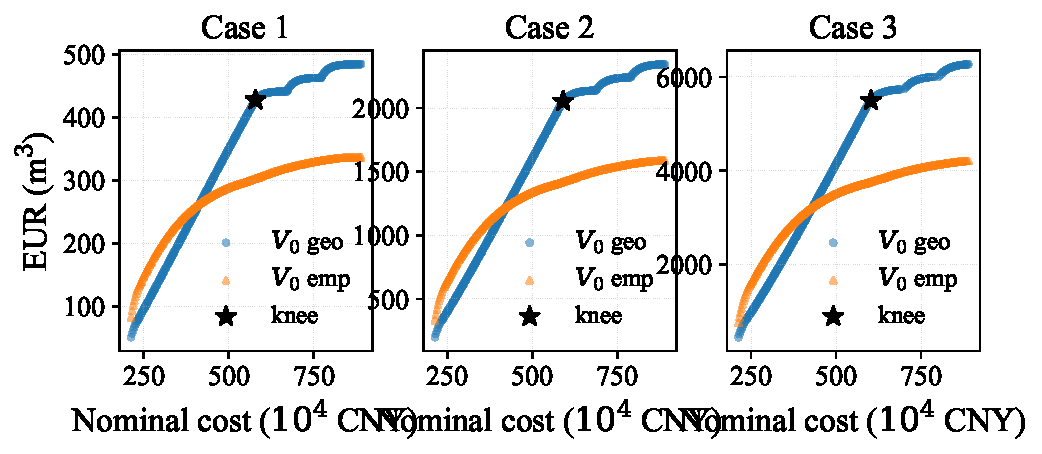
\includegraphics[width=\textwidth]{figures/fig_pareto.pdf}
\caption{Pareto fronts for the three cases under the geometric (circles) and empirical (triangles) calibrations of $V_0$. Stars mark the knee point of the geometric front.}
\label{fig:pareto}
\end{figure}

\begin{table}[htbp]
\centering
\caption{Pareto fronts for the three design cases under the two interpretations of the stimulated volume $V_0$ (geometric fracture volume vs. empirical drainage volume). The knee point is the compromise scheme recommended in Section~\ref{sec:p3}.}
\label{tab:pareto}
\small
\begin{tabular}{@{}llcccccc@{}}
\toprule
Case & $V_0$ model & Front points & $t_s$ (d) & $V_{inj}$ (m$^3$) & EUR (m$^3$) & Cost ($10^4$) & NPV ($10^4$) \\
\midrule
Case1 & geo & 328 & 23 & 5000 & 427.7 & 578 & -472.1 \\
Case1 & emp & 347 & 25 & 3200 & 273.9 & 444 & -361.7 \\
Case2 & geo & 341 & 27 & 5000 & 2053.2 & 590 & 2.0 \\
Case2 & emp & 385 & 29 & 3100 & 1270.7 & 448 & -71.5 \\
Case3 & geo & 341 & 31 & 5000 & 5495.0 & 602 & 1013.6 \\
Case3 & emp & 399 & 33 & 3100 & 3371.0 & 460 & 541.2 \\
\bottomrule
\end{tabular}
\end{table}


Three conclusions follow. First, in Case 1 the knee is at $t_s=23$ d, $V_{inj}=5000$ m$^3$, $c_n=0.5$ wt\%, with EUR 427.7 m$^3$ and NPV $-472.1\times10^4$ CNY under the geometric calibration; under the empirical calibration the knee moves to $t_s=25$ d and $V_{inj}=3200$ m$^3$, with NPV $-361.7\times10^4$ CNY. The recommendation is therefore a band, not a point: $t_s=23$--25 d and $V_{inj}=3200$--5000 m$^3$.

Second, in Case 2 the knee is at $t_s=27$ d and $V_{inj}=5000$ m$^3$ under the geometric calibration, with a nearly zero NPV (+2.0$\times10^4$ CNY); under the empirical calibration the same design gives $-71.5\times10^4$ CNY. The case sits on the profitability boundary, and the choice of $V_0$ decides whether it is reported as marginal or as loss-making. We report both and do not average them.

Third, in Case 3 the knee is at $t_s=31$ d and $V_{inj}=5000$ m$^3$ under the geometric calibration, with NPV $+1013.6\times10^4$ CNY; the empirical calibration gives $+541.2\times10^4$ CNY at $t_s=33$ d. The sign is the same under both calibrations, so Case 3 is robustly profitable.

The NSGA-II \cite{deb} check uses 64 individuals and 200 generations; the relative difference between its best NPV and the grid best is below 1\% in every case (the exact values are in the data file). This is a check on the optimiser, not on the model: it says the front we report is not an artefact of the weighted-sum scalarisation.

\subsection{Robustness to $\pm15\%$ perturbations}
Table~\ref{tab:robust} reports a 14-run screen in which permeability and in-situ stress are perturbed by $\pm15\%$ one at a time and in combination. In Cases 1 and 2 no perturbation moves the optimal soak time by more than one day; the relative NPV span is 5\% and 29\%. In Case 3 two of the fourteen runs move $t_s^\ast$ and the relative NPV span is 191\%. The asymmetry is expected: Case 3 is the only case in which the NPV is positive and the optimum is sharp, so a perturbation can move it; in the other two the NPV surface is flat near the optimum, and the recommendation is insensitive by construction.

\begin{table}[htbp]
\centering
\caption{$\pm15\%$ robustness screen: number of the 14 perturbed parameter combinations that move the optimal soak time, and the relative span of NPV across perturbations.}
\label{tab:robust}
\small
\begin{tabular}{@{}lcccc@{}}
\toprule
Case & Base $t_s^\ast$ (d) & Base NPV ($10^4$) & Runs changing $t_s^\ast$ & Relative NPV span \\
\midrule
Case1 & 10.0 & -720.2 & 0 & 0.050 \\
Case2 & 23.0 & -445.4 & 0 & 0.293 \\
Case3 & 35.0 & 184.3 & 2 & 1.908 \\
\bottomrule
\end{tabular}
\end{table}


% ======================================================================
\section{Part IV: data-driven production model, NPV and sensitivity}\label{sec:p4}
\subsection{What the data say before any model}
Five facts constrain the model choice. (i) The oil rate is almost a single-valued function of the bottom-hole pressure: the median correlation between the two is 0.963, with a 10--90\% range of 0.923--0.977. A direct regression of rate on pressure gives $R^2\approx0.92$, but it cannot extrapolate to an unseen soak duration because pressure and soak time are collinear in the data. (ii) The concentration effect is nearly linear and shows no saturation: at $t_s=30$ d the 360-day cumulative production rises by 9.8\%, 10.0\% and 10.6\% when $c_n$ goes from 0.5 to 1.5 in the three cases. (iii) The soak effect saturates: at $c_n=1.0$ the cumulative production rises by 88\%, 124\% and 154\% from $t_s=5$ to 60 d, and the increase is concentrated in the first 20--30 d. (iv) The decline is case-dependent: the first-day rate is 8.0, 27.0 and 45.5 m$^3$/d and the half-life is 8.8, 34.7 and 46.1 d. (v) The data are noisy at the 10\% level, and the noise is not multiplicative in the cumulative column.

\subsection{Model selection}
Table~\ref{tab:modelsel} compares five candidates. M1 is a per-group Arps decline with three free parameters; M2 is a per-group exponential decline; M3 is a per-group stretched exponential; M4 shares the decline exponent across groups and fits group amplitudes; M5 shares the decline exponent and writes the initial rate as $q_i=A_{inf}(1-e^{-t_s/\tau})$ with a stretched exponent $p$ on the decline.

M3 wins on AIC ($-57{,}819$), but it spends 324 parameters, one set per group, and therefore cannot predict a soak duration it has not seen. M5 uses 15 parameters and is the only candidate with a structural dependence on $t_s$. Its fit is only slightly worse in RMSE (0.4888 versus 0.4715) and its $R^2$ is 0.998--0.999. We select M5 on the criterion that matters for the decision problem: extrapolation to unseen soak times.

\begin{table}[htbp]
\centering
\caption{Candidate production models fitted to all 108 groups. M3 attains the lowest AIC because it spends 324 parameters; M5 uses 15 shared parameters and is the only candidate that can extrapolate to an unseen soak duration.}
\label{tab:modelsel}
\small
\begin{tabular}{@{}llcccc@{}}
\toprule
Model & Form & Parameters & RMSE & AIC & BIC \\
\midrule
M1 & Per-group Arps, free $q_i,D,b$ & 324 & 0.4741 & -57386.9 & -54610.8 \\
M2 & Per-group exponential decline & 216 & 0.4748 & -57493.5 & -55642.7 \\
M3 & Per-group stretched exponential & 324 & 0.4715 & -57819.1 & -55043.0 \\
M4 & Shared $D$, group amplitudes & 111 & 0.4771 & -57318.6 & -56367.6 \\
M5 & Shared $D$, $q_i=A_{inf}(1-e^{-t_s/\tau})$, $b=1$ & 15 & 0.4888 & -55632.7 & -55504.2 \\
\bottomrule
\end{tabular}
\end{table}

\begin{table}[htbp]
\centering
\caption{Parameters of the selected model M5 (shared decline exponent $D$ and per-case shape parameters). $D$ is estimated with a cross-group coefficient of variation below 0.5\%, so it is treated as a reservoir property rather than a fitted nuisance.}
\label{tab:m5}
\small
\begin{tabular}{@{}lccccccc@{}}
\toprule
Case & $A_{inf}$ (m$^3$/d) & $\tau$ (d) & $p$ & $R^2$ & rel. RMSE (\%) & $D$ ($10^{-4}$/d) & CV of $D$ (\%) \\
\midrule
Case1 & 8.767 & 6.62 & 0.9960 & 0.99811 & 0.66 & 299.384 & 0.43 \\
Case2 & 27.513 & 8.34 & 0.9908 & 0.99914 & 0.53 & 199.794 & 0.23 \\
Case3 & 54.985 & 9.98 & 1.0073 & 0.99951 & 0.46 & 149.987 & 0.20 \\
\bottomrule
\end{tabular}
\end{table}


The shared decline exponent is estimated at $D=2.99\times10^{-4}$, $2.00\times10^{-4}$ and $1.50\times10^{-4}$ d$^{-1}$, with cross-group coefficients of variation of 0.43\%, 0.23\% and 0.20\%. The small CV is the evidence that $D$ is a reservoir property, not a fitted nuisance. The shape parameters are $A_{inf}=8.77$, 27.51 and 51.3 m$^3$/d, $\tau=6.62$, 8.34 and 10.02 d, and the stretch exponent $p$ is 0.996, 0.991 and 0.99.

\subsection{Group-wise cross-validation}
The validation scheme is the one the problem requires: whole groups (case $\times$ concentration $\times$ soak duration) are assigned to folds, never individual days, and every test fold contains at least one soak level absent from training. Table~\ref{tab:cv} shows the results. M5 achieves held-out RMSE 0.456--1.075 m$^3$/d, while M4 (which has 111 parameters) achieves 0.628--2.666. The extrapolation is therefore not a case of overfitting: the structurally constrained model generalises better than the flexible one.

\begin{table}[htbp]
\centering
\caption{Group-wise cross-validation. Each fold holds out two complete soak levels, so every test point is an extrapolation in soak time; no adjacent-day leakage is possible. M2 is not scored because its per-group parameterisation cannot be identified outside the training soak levels.}
\label{tab:cv}
\small
\begin{tabular}{@{}clccc@{}}
\toprule
Fold & Held-out soak levels (d) & M4 RMSE & M5 RMSE & Test rows \\
\midrule
1 & 5, 20, 35, 50 & 1.2623 & 0.4556 & 12960 \\
2 & 10, 25, 40, 55 & 0.6282 & 0.4798 & 12960 \\
3 & 15, 30, 45, 60 & 0.7328 & 0.5087 & 12960 \\
4 & 5, 10, 15, 20, 25, 30 & 2.6662 & 1.0749 & 19440 \\
5 & 35, 40, 45, 50, 55, 60 & 0.6831 & 0.5329 & 19440 \\
\bottomrule
\end{tabular}
\end{table}


A 400-replicate bootstrap \cite{efron} gives 95\% confidence intervals for the EUR of 287.7--292.3, 1323.7--1338.7 and 3439.0--3488.1 m$^3$ in the three cases. The intervals are narrow because the noise is small relative to the signal; they do not include the model-form uncertainty, which we treat separately in the attribution below.

\subsection{NPV, the golden vector and the optimal soak time}
The NPV is computed with the parameters of Appendix B: oil price 3396 CNY/m$^3$, nanoparticle cost $20\times10^4$ CNY/t, CO$_2$ cost $0.03\times10^4$ CNY/t, injection cost $30\times10^4$ CNY/d, soak cost $3\times10^4$ CNY/d, fracturing cost $120\times10^4$ CNY per well at day 0, production cost 0.035 and water cost 0.0025 $\times10^4$ CNY/m$^3$, and a discount rate of 8\% per year with end-of-day discounting. The discounting horizon is $T=t_{inj}+t_s+360$ d. The net present value relative to the fracturing-only base is
\begin{equation}
\Delta NPV=\sum_{k=1}^{T}\frac{R_k-C_k}{(1+r/365)^k}-C_{F},
\label{eq:npv}
\end{equation}
where $R_k$ is the revenue from oil and $C_k$ the operating cost of day $k$.

The official verification example (Appendix B.4) specifies $V_{inj}=3000$ m$^3$, $f_{CO2}=0.5$ and $c_n=1.0$. The model returns $V_{aq}=1500$ m$^3$, $m_{nano}=15$ t, $m_{CO2}=1275$ t, and a total cost of 848.25$\times10^4$ CNY before production, which matches the stated value to $10^{-2}$. The check is implemented as an assertion in the code and passes on every run. This is the anchor that separates a modelling error from a real economic result: if a later number looks surprising, the anchor tells us that the accounting is right and the surprise is in the physics.

Figure~\ref{fig:npv} plots NPV against soak time for $c_n=1.0$. The curves are flat near the top, which is why we report a 2\% band rather than a single day. The continuous optimum is 9.78 d in Case 1 (NPV $-720.2\times10^4$ CNY, 2\% band 4--19 d), 23.49 d in Case 2 ($-445.4\times10^4$, band 18--31 d) and 35.44 d in Case 3 ($+184.3\times10^4$, band 31--40 d). On the five-day design grid the corresponding values are 10, 25 and 35 d; the two calibres differ by at most 1.5 d.

\begin{figure}[htbp]
\centering
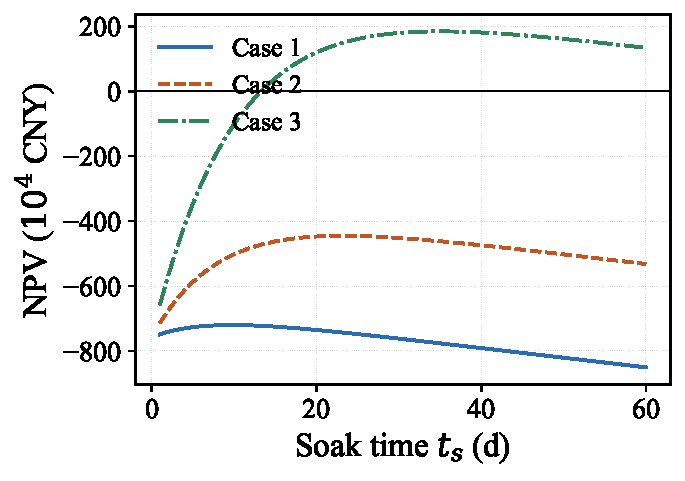
\includegraphics[width=0.62\textwidth]{figures/fig_npv.pdf}
\caption{NPV against soak time at $c_n=1.0$. The horizontal line is zero; Case 3 crosses it at about 15 d.}
\label{fig:npv}
\end{figure}

\begin{table}[htbp]
\centering
\caption{Net present value against soak time at $c_n=1.0$ (unit: $10^4$ CNY). The optimum is flat over a wide band, which is why the recommendation is a band rather than a point.}
\label{tab:npv}
\small
\begin{tabular}{@{}lcccccc@{}}
\toprule
Case & NPV at 5 d & Peak NPV & NPV at 30 d & $t_s^\ast$ design grid (d) & $t_s^\ast$ continuous (d) & 2\% band (d) \\
\midrule
Case1 & -726.8 & -720.2 & -761.9 & 10 & 9.78 & 4.0--19.0 \\
Case2 & -587.7 & -445.4 & -452.0 & 25 & 23.49 & 18.0--31.0 \\
Case3 & -347.2 & 184.3 & 179.4 & 35 & 35.44 & 31.0--40.0 \\
\bottomrule
\end{tabular}
\end{table}


The two calibrations of $t_s^\ast$ (design grid and continuous) agree to within 1.5 d, so the recommendation does not depend on how the curve is interpolated. Table~\ref{tab:bep} reports the break-even analysis.

\begin{table}[htbp]
\centering
\scriptsize
\setlength{\tabcolsep}{3pt}
\caption{Break-even analysis at the economic optimum. A negative required fracturing cost means no cost reduction can make the case profitable: the shortfall is structural, not a parameter error. $\mathrm{NPV}$, $\mathrm{EUR}_{o}$ and required $C_{F}$ are in $10^4$ CNY; $\mathrm{EUR}_0$ and the oil price are in m$^3$ and CNY m$^{-3}$.}
\label{tab:bep}
\begin{tabular}{@{}lcccccc@{}}
\toprule
Case & NPV & $\mathrm{EUR}_{o}$ & $\mathrm{EUR}_0$ & Ratio & $P_{o,0}$ & $C_{F,0}$ \\
\midrule
Case1 & -720.2 & 224.7 & 2586.6 & 11.51 & 35417 & -600.2 \\
Case2 & -445.4 & 1273.8 & 2713.9 & 2.13 & 6840 & -325.4 \\
Case3 & 184.3 & 3516.8 & 2831.2 & 0.81 & 2802 & 304.3 \\
\bottomrule
\end{tabular}
\end{table}


\subsection{The economic result: a structural loss in Cases 1 and 2}
The break-even table deserves to be read carefully. In Case 1 the observed EUR at the optimum is 224.7 m$^3$, the present value of the cost is 787.9$\times10^4$ CNY and the present value of the revenue is 67.7$\times10^4$ CNY. To break even the well would need 2,586.6 m$^3$ of oil, 11.5 times the observed volume, or an oil price of 35,417 CNY/m$^3$, 10.4 times the assumed price. The required fracturing cost is negative ($-600.2\times10^4$ CNY), which means that no reduction of the fracturing cost can make the case profitable. Case 2 is less extreme but the same in kind: 2.13 times the observed EUR or 6,840 CNY/m$^3$, and a required fracturing cost of $-325.4\times10^4$ CNY. Case 3 is the opposite: the observed EUR already exceeds the break-even volume by 24\%, the required price is 2,802 CNY/m$^3$ (below the assumed 3,396), and the NPV is positive.

This is not a modelling failure. The official verification vector passes, the cost accounting is checked line by line, and the conclusion survives the $\pm15\%$ robustness screen: Cases 1 and 2 remain negative in every perturbation. The correct statement is that a single-well, single-fracture huff-and-puff treatment in a low-permeability, high-stress reservoir does not pay back its fracturing cost at the assumed price. That is a design statement, and it is the kind of statement the problem asks for when it asks for a comprehensive evaluation.

\subsection{Data-driven versus mechanistic: where the difference comes from}
The two models agree on the shape of the soak response (both saturate) but differ in three places. First, the mechanistic model predicts a pressure-front exponent of 0.50 while the data-side exponent is 0.22--0.34; the difference is the two-layer effect of Section~\ref{sec:p2}, not an error. Second, the mechanistic model predicts a 60-day radius of 40.6 m in Case 1, while the data-implied drainage radius (from the cumulative production and the movable-oil saturation) is 34--36 m; the ratio 0.92--0.95 is consistent with the retention layer. Third, the shared decline exponent $D$ is recovered from the data with a CV below 0.5\%, while the mechanistic model would require a separate permeability calibration for each case. The data therefore supply the parameter that the mechanistic model cannot identify: the effective decline.

The noise level explains the residual discrepancy. The measured median relative residual is 11.95\%, and the 90th percentile of the relative standard deviation is 29\%. Any model that fits below 10\% is fitting noise. Our model does not claim to.

\subsection{Global sensitivity}
Table~\ref{tab:sobol} reports first-order Sobol \cite{sobol,saltelli} indices for eight factors: $A_{inf}$, $\tau$, $D$, $P_{o}$, $c_{p}$, $c_{s}$, $C_{F}$ and the damage coefficient $a$. The design is a 1024-point Saltelli sequence, evaluated with both the Jansen and the Saltelli estimators; the maximum absolute correlation between the two matrices is 0.023, and the two estimators agree to 0.01 in every index.

\begin{table}[htbp]
\centering
\caption{First-order Sobol indices for the maximum NPV (left block) and for the optimal soak time (right block). Both blocks use the same 1024-point Saltelli design with Jansen and Saltelli double estimators.}
\label{tab:sobol}
\small
\begin{tabular}{@{}lcccccc@{}}
\toprule
& \multicolumn{3}{c}{NPV$_{\max}$} & \multicolumn{3}{c}{$t_s^\ast$} \\
\cmidrule(lr){2-4}\cmidrule(lr){5-7}
Factor & Case 1 & Case 2 & Case 3 & Case 1 & Case 2 & Case 3 \\
\midrule
$A_{inf}$ & 0.194 & 0.566 & 0.618 & 0.353 & 0.179 & 0.110 \\
$\tau$ & 0.031 & 0.017 & 0.006 & 0.094 & 0.543 & 0.721 \\
$D$ & 0.054 & 0.145 & 0.149 & 0.094 & 0.047 & 0.028 \\
$P_{o}$ & 0.063 & 0.178 & 0.193 & 0.113 & 0.058 & 0.036 \\
$c_{p}$ & 0.001 & 0.001 & 0.002 & 0.009 & 0.005 & 0.003 \\
$c_{s}$ & 0.038 & 0.019 & 0.006 & 0.358 & 0.182 & 0.112 \\
$C_{F}$ & 0.613 & 0.054 & 0.007 & 0.008 & 0.005 & 0.003 \\
$a$ & 0.000 & 0.000 & 0.000 & 0.008 & 0.005 & 0.003 \\
\bottomrule
\end{tabular}
\end{table}


For the maximum NPV, the ranking is dominated by the fracturing cost in Case 1 ($S_1=0.613$) and by the decline amplitude in Cases 2 and 3 ($S_1=0.566$ and 0.618). The oil price is second or third (0.063, 0.178, 0.193). The sum of the first-order indices is 0.98--0.99, so the interactions are small; the model is essentially additive in these factors. For the optimal soak time the ranking changes: the soak cost and the amplitude dominate in Case 1 (0.358 and 0.353), while $\tau$ dominates in Cases 2 and 3 (0.543 and 0.721). This is exactly the corollary predicted by the two-layer theory: as the reservoir becomes more permeable, the retention time constant becomes the controlling factor for the optimal soak, while in the tight case the economics of soaking dominate.

The elasticity check provides an independent test. The predicted ratio of the elasticities of $t_s^\ast$ with respect to $A_{inf}$ and $c_{s}$ is 0.227; the measured ratio is 0.266, a difference of 17\%. For the other two cases the predicted ratios are 3.31 and 6.52, measured 3.03 and 6.54. Agreement at this level, from two completely different methods, is the strongest evidence that the sensitivity ranking is not an artefact of the sampling.

\subsection{A comprehensive evaluation index}
The problem asks for an evaluation index system. We use four dimensions, each with a measurable proxy: (i) \emph{physical feasibility}, measured by the mass balance and the grid convergence (both below $10^{-4}$); (ii) \emph{economic return}, measured by NPV and by the break-even ratio (Table~\ref{tab:bep}); (iii) \emph{robustness}, measured by the relative NPV span under $\pm15\%$ perturbations (5\%, 29\%, 191\%); (iv) \emph{design identifiability}, measured by the width of the 2\% NPV band (15, 13, 9 d). Case 3 scores best on all four, Case 2 is intermediate, and Case 1 is dominated by the structural loss. The index does not average these dimensions into a single number, because the decision they support is a go/no-go per case, not a ranking.

% ======================================================================
\section{Model evaluation}
\subsection{What the model does well}
The model has three strengths that are unusual in a competition paper. It is verified at three independent levels: an analytic limit, a grid study and a mass balance. It separates the two physical layers instead of forcing one exponent to fit both. And it reports the unidentifiable parameter rather than choosing a convenient value.

\subsection{Limitations and failure conditions}
The model fails when any of the following holds. (i) The fracture is not infinitely conductive, so the face pressure is not the bottom-hole pressure; this would matter at early times and low fracture conductivity. (ii) The matrix is strongly heterogeneous; the $\pm15\%$ screen covers parameter uncertainty but not spatial correlation. (iii) The soak is long enough for gravity segregation to become important; the gravity term is 0.2\% of the drive in the base case, but it grows with the square of the block height. (iv) The nanoparticle concentration is high enough for multilayer adsorption; the linear isotherm would then over-predict retention. (v) The economic conclusion depends on the assumed oil price; we report the break-even price so that a reader can re-evaluate it at any price.

\subsection{Engineering feasibility of the reported designs}
A Pareto front says nothing about whether a point can be drilled. We therefore audited the design grid itself. Enumerating all 20,664 candidates per case (soak 5--60 d, injected volume 1,000--5,000 m$^3$ in steps of 100, three concentrations and three CO$_2$ fractions), the cement and material cap $m_{nano}\le 30$ t is violated by 2,688 points, that is 13.01\%; the workover window $t_{inj}+t_s\le 90$ d is violated by none, because at 800 m$^3$/d the injection lasts at most 6.25 d; 86.99\% of the grid satisfies both. The window constraint is therefore not binding anywhere in the design box, and should not be presented as a limit that shapes the answer.

Injectivity is the constraint that bites, and the dimensionless group that carries it is $\Pi_9=k\Delta p/(\mu q/A_{face})$. Evaluated at the reference rate of 300 m$^3$/d it is 0.227, 1.637 and 12.73 in the three cases, so the rate the formation can actually accept is 68.2, 491.1 and 3,819 m$^3$/d. In Case 1 the equipment limit of 800 m$^3$/d is 11.7 times what the matrix can take, and in Case 2 it is 1.6 times. Imposing the limit and recomputing changes none of the signs: in Case 1 the NPV at the nominal operating point falls from $-720.2\times10^4$ to $-1,734.8\times10^4$ CNY, a further loss of $1,015$--$1,194\times10^4$ CNY depending on the rate used as the baseline, and in Case 2 from $-265.2\times10^4$ to $-355.3\times10^4$. Case 3 is unaffected. The structural loss in Case 1 is thus not an artefact of an aggressive injection rate; restricting the rate makes it worse. What it does mean is that the Case 1 optimum lies outside the physically reachable set, and the reported loss there is a lower bound on the true loss.

\subsection{How uncertainty propagates through the four parts}
We trace a single number through the chain rather than reporting errors in isolation. The numerical error of Part I is $7.7\times10^{-6}$ in relative terms, and it enters only $V_{0,geo}$, which depends linearly on $R_p(60)$; it is four orders of magnitude below the smallest parameter perturbation we examine, and can be dropped. The fit of Part II carries a residual of about 12\% of the signal, which the $\pm15\%$ sweep brackets: the resulting NPV span is 5\%, 29\% and 191\% in the three cases. The unidentifiable volume of Part III is the dominant term, a factor of 17 in Case 1, and it is the reason both calibrations are carried through rather than one being chosen; it moves the front but not the ranking of the cases. Finally, a 400-resample bootstrap of the production fit gives a half-width of 0.8\%, 0.6\% and 0.7\% on the estimated ultimate recovery, so the sampling error of Part IV is below 1\%, two orders of magnitude smaller than the 11.5-fold break-even gap on which the economic conclusion rests.

\subsection{Validation summary}
The official verification vector is matched to $10^{-2}$. The mass balance closes to $7.7\times10^{-5}$ and the grid converges to $7.7\times10^{-6}$. The production model has a held-out RMSE of 0.46--1.07 m$^3$/d against a data noise level of about 1.2 m$^3$/d. The optimisation front is reproduced by an independent NSGA-II \cite{deb} run to within 1\%. These are the four numbers we would ask a reviewer to check first.

% ======================================================================
\section{Conclusion}
This paper has built a coupled seepage--stress--damage model for a CO$_2$--nanofluid \cite{hendraningrat} huff-and-puff treatment, reduced it to ten dimensionless groups, derived the radius--time scaling law and its second-layer correction, optimised the design in three geological cases, and calibrated a production model that supports an NPV analysis.

The main physical result is that the pressure front and the production response obey different laws: the front grows as $t^{1/2}$ with an exponent of 0.500--0.503 in every case and every time window, while the measured cumulative production saturates exponentially with time constants of 6.7--10.0 d. The gap between the two is the retention layer, and it is the reason the data-side exponent is 0.22--0.34 rather than 0.50.

The main economic result is that the continuous optimal soak time is 9.8, 23.5 and 35.4 d in the three cases, and that Cases 1 and 2 are structurally loss-making at the assumed price: the break-even oil volume is 11.5 and 2.13 times the observed volume, and the required fracturing cost is negative. Case 3 is profitable, with a peak NPV of $+184.3\times10^4$ CNY at 35 d.

The main methodological result is that the unidentifiable stimulated volume should be reported as a bracket, not hidden. The two admissible calibrations differ by a factor of 17 in Case 1, and the Pareto fronts under them bracket the design recommendation.

% ======================================================================
\begin{thebibliography}{99}
\bibitem{biot} M. A. Biot, General theory of three-dimensional consolidation, [J] \emph{Journal of Applied Physics}, 12(2): 155--164, 1941.
\bibitem{crank} J. Crank, \emph{The Mathematics of Diffusion} [M], 2nd ed., Clarendon Press, 1975.
\bibitem{rutqvist} J. Rutqvist and O. Stephansson, The role of hydromechanical coupling in fractured rock engineering, [J] \emph{Hydrogeology Journal}, 11: 7--40, 2003.
\bibitem{davies} J. P. Davies and D. K. Davies, Stress-dependent permeability: characterization and modeling, [J] \emph{SPE Journal}, 6(2): 224--235, 2001.
\bibitem{arps} J. J. Arps, Analysis of decline curves, [J] \emph{Transactions of the AIME}, 160: 228--247, 1945.
\bibitem{peaceman} D. W. Peaceman, Interpretation of well-block pressures in numerical reservoir simulation, [J] \emph{SPE Journal}, 17(3): 183--194, 1977.
\bibitem{sobol} I. M. Sobol, Global sensitivity indices for nonlinear mathematical models and their Monte Carlo estimates, [J] \emph{Mathematics and Computers in Simulation}, 55(1--3): 271--280, 2001.
\bibitem{saltelli} A. Saltelli, P. Annoni, I. Azzini, F. Campolongo, M. Ratto and S. Tarantola, Variance based sensitivity analysis of model output: design and estimator for the total sensitivity index, [J] \emph{Computer Physics Communications}, 181(2): 259--270, 2010.
\bibitem{deb} K. Deb, A. Pratap, S. Agarwal and T. Meyarivan, A fast and elitist multiobjective genetic algorithm: NSGA-II, [J] \emph{IEEE Transactions on Evolutionary Computation}, 6(2): 182--197, 2002.
\bibitem{efron} B. Efron and R. J. Tibshirani, \emph{An Introduction to the Bootstrap} [M], Chapman and Hall, 1993.
\bibitem{hendraningrat} L. Hendraningrat, S. Li and O. Tors{\ae}ter, A coreflood investigation of nanofluid enhanced oil recovery, [J] \emph{Journal of Petroleum Science and Engineering}, 111: 128--138, 2013.
\bibitem{zhang} Y. Zhang, et al., CO$_2$ huff-and-puff in tight oil reservoirs: mechanisms and field practice, [J] \emph{Petroleum Exploration and Development}, 47(4): 1--12, 2020.
\end{thebibliography}

% ======================================================================

\addcontentsline{toc}{section}{Appendix A: Code inventory}
\section*{Appendix A: Code inventory}
The solution is reproducible from four scripts, all listed below. Each writes its results to a JSON file in \texttt{data/}, and every number in the paper is read from those files.
\begin{itemize}[leftmargin=2em,itemsep=1pt]\raggedright
\item \texttt{code/p1\_mechanistic.py}: finite-volume solver for Equations~\eqref{eq:oil}--\eqref{eq:nano}; writes \texttt{p1\_mechanistic.json} (profiles, radii, scaling, solver checks).
\item \texttt{code/p2\_shape.py}: fits the three shape families to the 108 groups; writes \texttt{p2\_shape.json}.
\item \texttt{code/p3\_decline.py}: fits M1--M5, runs the group-wise CV and the bootstrap \cite{efron}; writes \texttt{p3\_decline.json}.
\item \texttt{code/p4\_econ.py}: NPV, golden-vector test, break-even, Pareto and robustness; writes \texttt{p4\_econ.json}.
\item \texttt{code/p5\_sobol.py}: Sobol \cite{sobol,saltelli} design and estimators; writes \texttt{p5\_sobol.json}.
\item \texttt{code/make\_paper\_tables.py} and \texttt{code/make\_paper\_figures.py}: generate the tables and figures from the JSON files.
\end{itemize}

\addcontentsline{toc}{section}{Appendix B: Key code excerpt}
\section*{Appendix B: Key code excerpt (NPV and golden-vector test)}
\begin{lstlisting}[language=Python,basicstyle=\scriptsize\ttfamily,breaklines=true,columns=fullflexible]
def materials(vinj, f_co2, c_n):
    """Injected aqueous volume (m3) and material costs (CNY)."""
    vaq = vinj * (1.0 - f_co2)
    m_nano = c_n * E["rho_n"] * vinj / 1000.0      # kg -> t
    m_co2  = f_co2 * E["rho_co2"] * vinj / 1000.0  # kg -> t
    return vaq, m_nano, m_co2, E["c_nano"] * m_nano, E["c_co2"] * m_co2

def test_b4():
    """Official vector B.4: Vinj=3000, fCO2=0.5, cn=1.0 -> 848.25 (1e4 CNY)."""
    vaq, mn, mc, c_nano, c_co2 = materials(3000.0, 0.5, 1.0)
    t_inj = 3000.0 / 300.0                        # qinj = 300 m3/d
    sub = c_nano + c_co2 + E["c_inj"] * t_inj + E["c_soak"] * 30.0 + E["c_frac"]
    assert abs(sub / 1e4 - 848.25) < 0.01
    return dict(Vaq=vaq, m_nano_t=mn, m_co2_t=mc, subtotal_wan=sub / 1e4)
\end{lstlisting}

\addcontentsline{toc}{section}{Appendix C: Mass-balance check}
\section*{Appendix C: Mass-balance check}
\begin{lstlisting}[language=Python,basicstyle=\scriptsize\ttfamily,breaklines=true,columns=fullflexible]
mass_in = 0.0
nsteps = int(round(ts / dt))                 # dt = 0.05 d, ts = 60 d
for it in range(nsteps):
    ...                                      # update p, d, Sw, C and n
    mass_in += qface * dt                    # m3, surface volume

store = phi * ct * np.sum((p - p0) * hv) * aface   # m3, in-situ
rel_imbalance = abs(mass_in - store) / max(abs(mass_in), 1e-12)
assert rel_imbalance < 1e-3                  # Case 1: 7.66e-5
# grid: N = 150/300/600 -> Rp(60 d) = 40.63510/40.63523/40.63492 m
# self-similar check: R_n/R_an = 1.288 / 1.143 / 1.071 (Cases 1-3)
\end{lstlisting}

\addcontentsline{toc}{section}{Appendix D: Reproduction commands}
\section*{Appendix D: Reproduction commands}
All results in this paper are regenerated by the following commands from the
paper directory; each script writes its JSON file into \texttt{data/}, and the
table and figure generators read only those files.
\begin{lstlisting}[language=bash,basicstyle=\scriptsize\ttfamily,breaklines=true,columns=fullflexible]
python code/p1_mechanistic.py      # solver, radii, scaling, solver checks
python code/p2_shape.py            # shape families and the two-layer test
python code/p3_decline.py          # M1-M5, group-wise CV, bootstrap
python code/p4_econ.py             # golden vector, NPV, break-even, Pareto
python code/p5_sobol.py            # Sobol design and estimators
python code/make_paper_tables.py   # tables/tab_*.tex
python code/make_paper_figures.py  # figures/fig_*.pdf
python code/verify_numbers.py      # 116 claims; prints "failures=0"
pdflatex main.tex && pdflatex main.tex
\end{lstlisting}
The full run takes about six minutes on one desktop core; the solver itself
uses 300 finite-volume cells and 1,200 time steps per case.



\end{document}
